
\part[Recursão]
{Recursão}


\chapter[Recursão]
{Recursão}



\section*{Resumo}

Recursão é uma sub-rotina que pode invocar a si mesma, contendo, a cada chamada, uma pedaço menor da solução final.

%\begin{chapreferences}{1.}
%\bibliography{playcb}
%\bibliographystyle{plain}
%\nocite{cbook}
%\nocite{sb6}
%\nocite{glfw}
%\nocite{cppbook}

%\end{chapreferences}

% \begin{chapreferences}{1}

% \bibitem{sb6}
% {\em OpenGL SuperBible}.
% \newblock Pearson Education Inc, 6 edition, 2014.

% \bibitem{glfw}
% Marcus Geelnard and Camilla Berglund.
% \newblock {\em GLFW - Reference guide}, 2010.
% \newblock API version 2.7.

% \bibitem{cbook}
% Brian~W. Kernighan and Dennis~M. Ritchie.
% \newblock {\em The C Programming Language}.
% \newblock 1989.

% \bibitem{cppbook}
% Stanley~B. Lippman, Josés Lajoile, and Barbara Moo.
% \newblock {\em C++ Primer}.
% \newblock 2013.
% \end{chapreferences}

\section*{Problemas}
\begin{enumerate}
\item
  Exiba passo a passo a solução da Torre de Hanói para, no máximo, 5 discos.
  \label{ex:cap04_ex1}

\item
  Sabendo que a curva de Koch é construída que toma, como base, um segmento de reta de tamanho $n$. Na extremidade deste primeiro segmento, desenha-se outro segmento de reta de tamanho $n$, porém com uma curvatura de $60º$ em relação ao primeiro. Na extremidade deste segundo segmento, desenha-se outra curva de reta de tamanho $n$, mas agora com a curvatura de $120º$ em relação ao primeiro. Por fim, desenha-se outro segmento de reta de tamanho $n$ na extremidade do terceiro segmento.
    \begin{enumerate}
      \item Exiba a curva de Koch de ordem $n$
        \label{ex:cap04_ex2a}
      \item Exiba um floco de neve de ordem $n$ baseado na curva de Koch
        \label{ex:cap04_ex2b}
    \end{enumerate}
  \label{ex:cap04_ex2}
\item
  A curva de Sierpiński preenche todo o espaço disponível sem cortar suas próprias linhas, sendo mutuamente recursiva entre quatro funções. AQUI TEM UMA EXPLICAÇÃO DAS REGRAS DESSA CURVA. Exiba a curva de Sierpiński de ordem $n$.
  \label{ex:cap04_ex3}
\end{enumerate}

\section*{Soluções}

\subsection*{Exercício \ref{ex:cap04_ex1} }
\begin{figure}[ht]
  \centerline{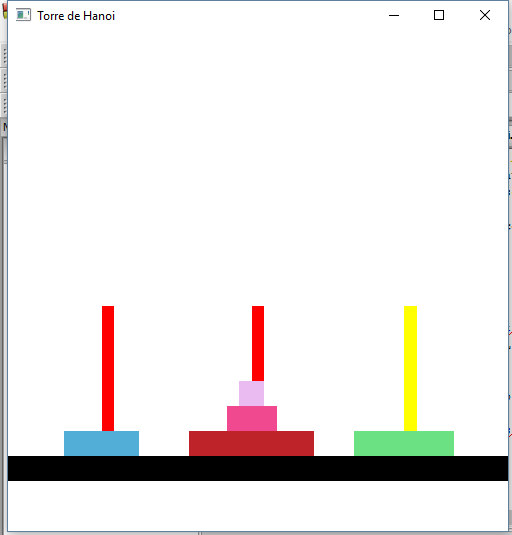
\includegraphics[width=.5\textwidth]{img/cap4_ex13.png}}
  \caption{Solucionador da torre de Hanói}
  \label{fig:cap04_ex1}
\end{figure}
Esta prática ilustra como mover cada geometria utilizando retorno da função \emph{CriaGrupo} para mover cada peça da torre de Hanoi para uma posição específica.
\lstinputlisting[caption=Código fonte da torre de Hanói, style=customc, label=lst:cap4_ex1]{src/ex13_hanoi.cpp}

\subsection*{Exercício \ref{ex:cap04_ex2} }
\subsubsection*{Item \ref{ex:cap04_ex2a}}
\begin{figure}[ht]
  \centerline{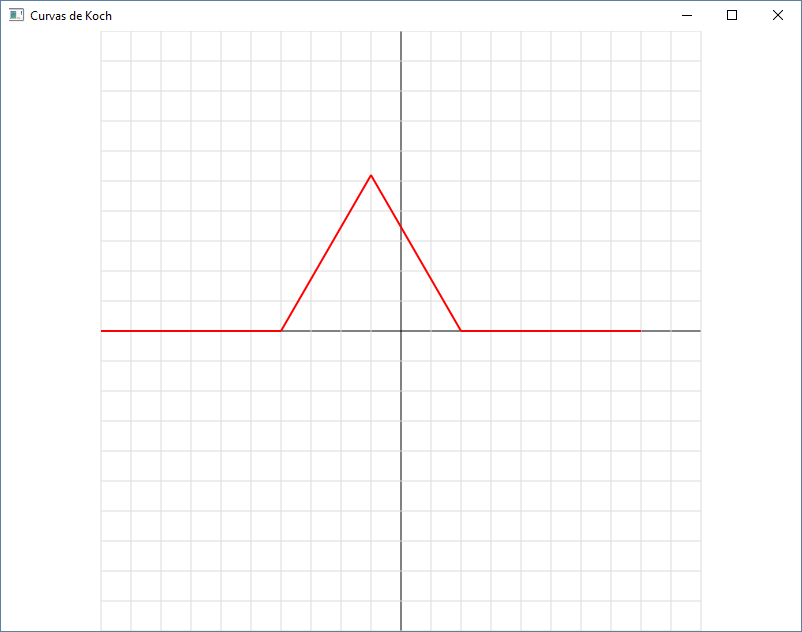
\includegraphics[width=.5\textwidth]{img/cap4_ex14.png}}
  \caption{Curva de Koch de ordem 3}
  \label{fig:cap04_ex2a}
\end{figure}
Esta prática reforça o modo de utilização da função CriaReta, usando a função \emph{movaCaneta}, na linha \ref{line:movaCaneta}.
\lstinputlisting[caption=Código fonte da curva de koch, style=customc, label=lst:cap4_ex1]{src/ex14_koch.cpp}

\subsubsection*{Item \ref{ex:cap04_ex2b}}
\begin{figure}[ht]
  \centerline{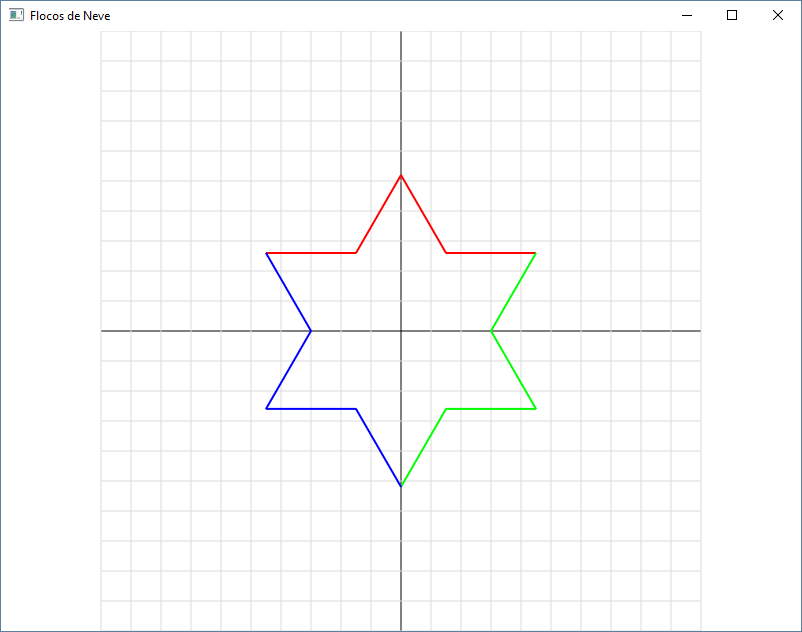
\includegraphics[width=.5\textwidth]{img/cap4_ex15.png}}
  \caption{Floco de neve}
  \label{fig:cap04_ex2b}
\end{figure}
\lstinputlisting[caption=Código fonte do floco de neve, style=customc, label=lst:cap4_ex1]{src/ex15_snowflake.cpp}


\subsection*{Exercício \ref{ex:cap04_ex3} }
\begin{figure}[ht]
  \centerline{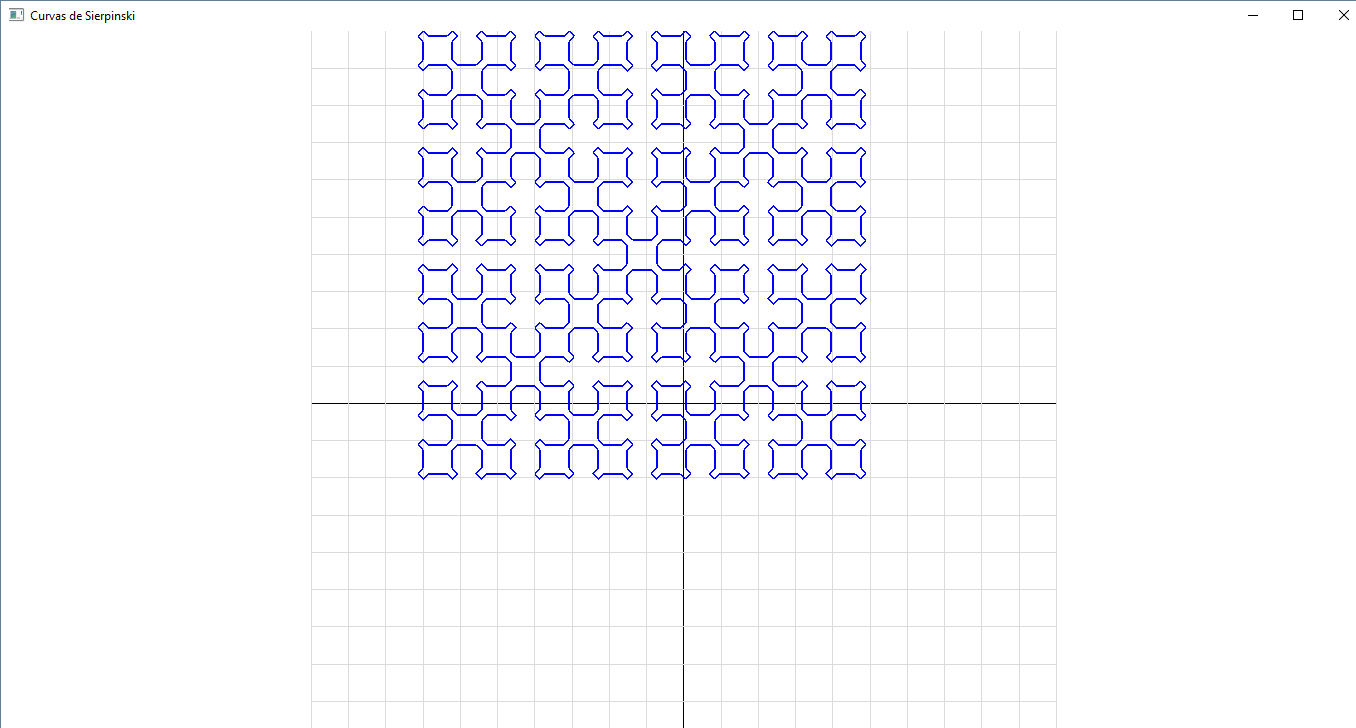
\includegraphics[width=.5\textwidth]{img/cap4_ex16.png}}
  \caption{Curva de Sierpiński}
  \label{fig:cap04_ex3}
\end{figure}
Esta prática reforça o modo de utilizar a função \emph{CriaReta}, usando as implementações das funções das linhas \ref{line:pontoA}, \ref{line:pontoB}, \ref{line:pontoC} e \ref{line:pontoD}.
\lstinputlisting[caption=Curva de Sierpiński, style=customc, label=lst:cap4_ex1]{src/ex16_sierpinski.cpp}